\section{Funktionsknoten}\label{anhang:funktionsknoten}
\begin{figure}[H]
\centering
\begin{subfigure}{.5\textwidth}
  \centering
  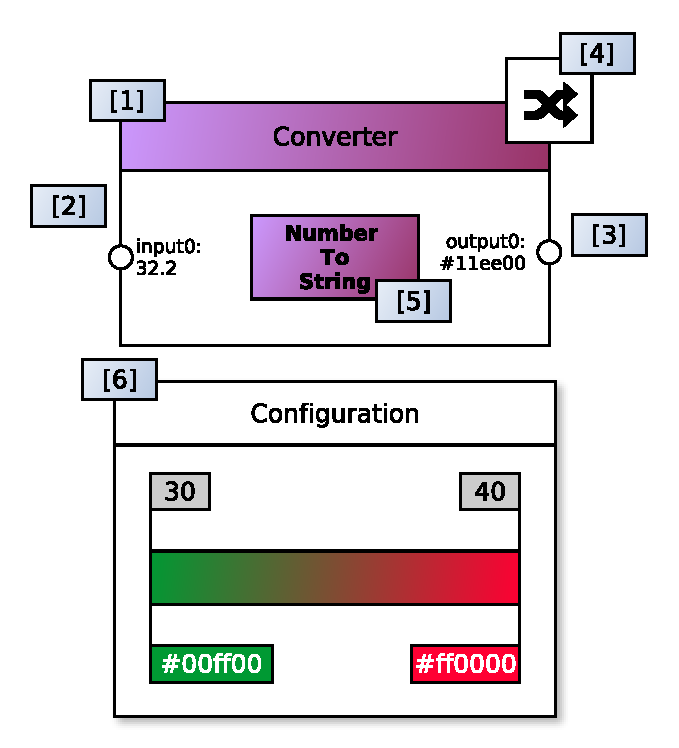
\includegraphics[width=1\linewidth]{bilder/Anhang/instanceconverterfunctionnode.pdf}
  \caption{Converter-Knoten: Bildet einen Definitionsbereich in einen Wertebereich ab.}
  \label{fig:funcconv}
\end{subfigure}%
\begin{subfigure}{.5\textwidth}
  \centering
  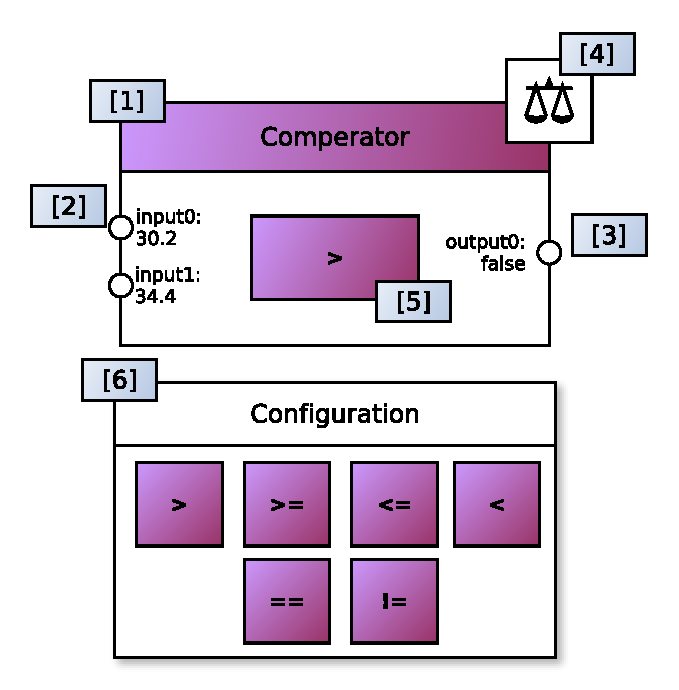
\includegraphics[width=1\linewidth]{bilder/Anhang/instancecomperatorfunctionnode.pdf}
  \caption{Comperator-Knoten: Vergleicht zwei \texttt{Number}-Werte und gibt einen Wahrheitswert weiter.}
  \label{fig:funccompare}
\end{subfigure}

\begin{subfigure}{.5\textwidth}
  \centering
  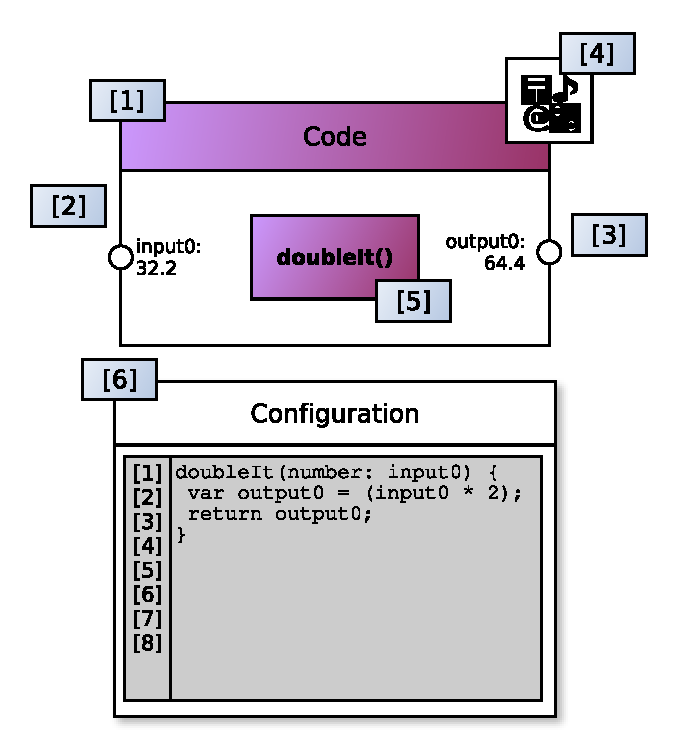
\includegraphics[width=1\linewidth]{bilder/Anhang/instancecodefunctionnode.pdf}
  \caption{Code-Knoten: Verarbeitet Daten anhand eines benutzerdefinierten Javascript-Programmcodes.}
  \label{fig:actorspecific}
\end{subfigure}%
\begin{subfigure}{.5\textwidth}
  \centering
  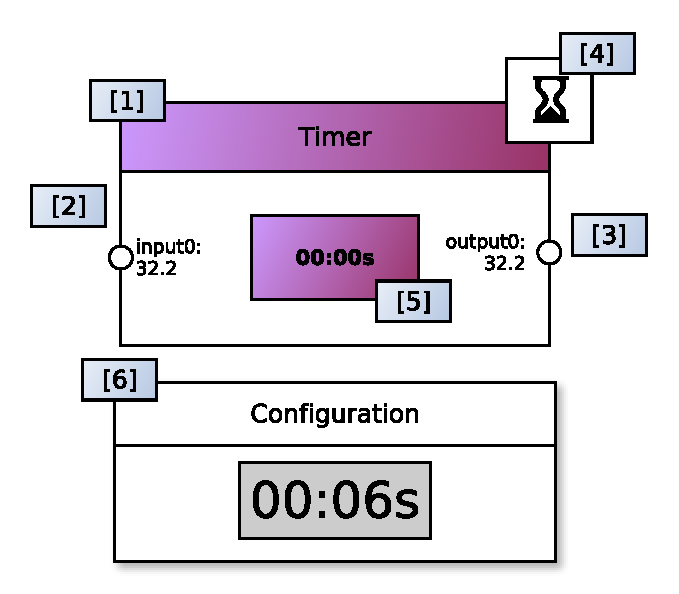
\includegraphics[width=1\linewidth]{bilder/Anhang/instancetimerfunctionnode.pdf}
  \caption{Timer-Knoten: Sendet das Eingangsignal nach einer benutzerdefinierten Zeitspanne weiter. [5] zeigt den momentanen Zustand des Timers an.}
  \label{fig:functimer}
\end{subfigure}

    \caption{Sammlung von verschiedenen Funktionsknoten. [1] Identifikationsleiste [2] Input-Schnittstellen [3] Output-Schnittstellen [4] Knoten-Indikator [5] Deskriptor [6] Knoten-Konfiguration}
    \label{fig:functionnodestypes}
\end{figure}